\documentclass{article}
\usepackage{tikz}
\usetikzlibrary{graphs,graphdrawing}
\usepackage{multirow}
\usepackage{multicol}
\usepackage{amsmath}

\usepackage{tkz-graph}
\usegdlibrary{trees}


\usepackage[margin=2cm]{geometry}

\usepackage[utf8]{inputenc}
\begin{document}
	\section{Esercitazione 2}
	
	\subsection{Esercizio 1}
	
	Consideriamo l’insieme di tutte le possibili mani di una partita a poker con 5
	carte, utilizzando un mazzo formato da 52 carte. 
	
	\begin{itemize}
		\item Quanti eventi atomici costituiscono la distribuzione di probabilità congiunta? 
	\end{itemize}

\[
\binom{52}{5} = 2.598.960
\]
	
		\begin{itemize}
		 \item	Qual è la probabilità di ciascun evento atomico? 
		\end{itemize}
\[
\frac{1}{2.598.960}
\]

		\begin{itemize}
	\item Qual è la probabilità di avere una scala reale?
\end{itemize}
\[
\frac{4}{2.598.960} = \frac{1}{649.740}
\]

		\begin{itemize}
	\item Qual è la probabilità di avere una scala reale?
\end{itemize}

\[
\frac{13 \cdot 48}{2.598.960} = \frac{1}{4.165}
\]

\pagebreak
\subsection{Esercizio 2}
Considerare questo grafo, quali tabelle di probabilità vanno specificate per fare sì che sia una reta bayesiana?
 \begin{center}
 	
	\begin{tikzpicture}
		\SetUpEdge[lw         = 1.5pt,
		color      = orange,
		labelcolor = white]
		\GraphInit[vstyle=Normal] 
		\SetGraphUnit{3}
		\tikzset{VertexStyle/.append  style={fill}}
		\Vertex{A}
		\SO(A){D}
		\SO(D){E}
		\WE(D){C}
		\SO(C){B}
		\EA(D){F}
		\tikzset{EdgeStyle/.style={->}}
		\Edge(B)(C)
		\Edge(B)(E)
		\Edge(C)(D)
		\Edge(D)(E)
		\Edge(A)(C)
		\Edge(A)(D)
		\Edge(A)(F)
		\Edge(F)(E)
	\end{tikzpicture}
\end{center}

\(P(A)\), \(P(B)\) , \(P(C | A, B)\) , \(P(D | A, C)\), \(P(E | B, D, F)\),  \(P(F | A)\)
\\
\vspace{0.3cm}
Qual è la markov blanket di ciascun nodo?

\textit{La markov blanket di un nodo è costituita dai suoi genitori, dai suoi figli e dai genitori dei figli. Un nodo non rientra mai nella sua coperta di markiv}

 \[A = { C, D, F, B }\]
 \[B = { C, E, A, F, D }\]
 \[C = { A, B, D }\]
 \[D = { A, C, E, F, B }\]
 \[E = { B, F, D }\]
 \[F = { A, D, B }\]
 
 \pagebreak
\subsection{Esercizio 3}

Data la seguente rete bayesiana, indicare quali affermazioni sono vere o false per indicare se due nodi sono condizionalmente indipendenti. \\

\begin{center}
\begin{tikzpicture}
	\SetUpEdge[lw         = 1.5pt,
	color      = orange,
	labelcolor = white]
	\GraphInit[vstyle=Normal] 
	\SetGraphUnit{3}
	\tikzset{VertexStyle/.append  style={fill}}
	\Vertex{A}
	\NOWE(A){B}
	\SOEA(A){M}
	\SOWE(A){J}
	\NOEA(A){E}
	\tikzset{EdgeStyle/.style={->}}
	\Edge(B)(A)
	\Edge(E)(A)
	\Edge(A)(J)
	\Edge(A)(M)
\end{tikzpicture}
\end{center}

\begin{itemize}
	\item \( B \bot M\) ?
	Falso, perchè  fra \(B\) e \(M\) c'è una connessione seriale (B -> A -> M) .
	Se A fosse osservato allora B e M sono indipendenti.
	
 \end{itemize}

\begin{itemize}
	\item \( J \bot M\ | A \) ?
	Vero, perchè abbiamo una connessione divergente e sappiamo il valore di A.
	(Sapere se l'allarme è in funzione  o meno non cambia il fatto che se Mary stia chiamando non ho modifiche sullale probabilità che anche John stia chiamando).

\end{itemize}

\begin{itemize}
	\item \( E \bot B\ | M \) ?
	Falso, se considero (B -> A <- M) c'è evidenza per un discendente di A (M) per cui non posso applicare la terza regola di d-seperazione.
	
\end{itemize}

\pagebreak

\subsection{Esercizio 4}

Data la seguente rete bayesiana, indicare quali affermazioni sono vere o false per indicare se due nodi sono condizionalmente indipendenti.


\begin{center}
	\begin{tikzpicture}
		\SetUpEdge[lw         = 1.5pt,
		color      = orange,
		labelcolor = white]
		\GraphInit[vstyle=Normal] 
		\SetGraphUnit{3}
		\tikzset{VertexStyle/.append  style={fill}}
		\Vertex{Creative}
		\EA(Creative){Smart}
		\SO(Creative){Project}
		\EA(Project){Mac}
		\EA(Mac){HW}
		\NOEA(HW){Party}
		\SO(Mac){Success}
		\EA(Success){Happy}
		\tikzset{EdgeStyle/.style={->}}
		\Edge(Creative)(Project)
		\Edge(Creative)(Mac)
		\Edge(Smart)(Project)
		\Edge(Smart)(Mac)
		\Edge(Smart)(HW)
		\Edge(Party)(HW)
		\Edge(Party)(Happy)
		\Edge(Project)(Success)
		\Edge(Mac)(Happy)
		\Edge(HW)(Success)
		\Edge(Success)(Happy)
		
	\end{tikzpicture}
\end{center}

\begin{itemize}
	\item \(Party \; \bot \; Success \;|\; HW\)
	\item \(Party \; \bot \; Smart \;|\; Success\)
	\item \(Party \; \bot \; Creative \;|\; Happy \)
\end{itemize}

\vspace{0.4cm}
\begin{itemize}
	\item \(Party \; \bot \; Success \;|\; HW\) \\
	Falso, c'è un cammino non bloccato che è (Party -> HW <- Smart -> Project -> Success)
\end{itemize}

\begin{itemize}
	\item \(Party \; \bot \; Smart \;|\; Success\)
	Falso, perchè il cammino Party -> HW <- Smart non è bloccato (Un discendente di HW, ovvero Success ha evidenza)
\end{itemize}

\begin{itemize}
	\item \(Party \; \bot \; Creative \;|\; Happy \)
	Falso, perchè il cammino Party -> Happy <- Mac <- Creative  non è bloccato
\end{itemize}


\pagebreak

\subsection{Esercizio 5}

Supponiamo che le variabili \(X_1, \; X_2, \; ..., \; X_K \) non abbiano un genitore in una determinata rete Bayesiana che contiene n variabili in tutto, dove n > k \\
La rete Bayesiana asserisce che \(P(X_1, X_2, ..., X_K) = P(X_1) \cdot P(X_2) ... P(X_K) \) \\.

L'affermazione è vera perchè se le variabili non hanno genitori (i nodi non hanno archi entranti) allora sono indipendenti , per cui la probabilità che siano tutte vere è calcolata come la probabilità di eventi indipendenti.

Un nodo è indipendente dai suoi predecessori dati i suoi genitori.

\pagebreak

\subsection{Esercizio 6}
Sia \(H_X\) una variabile casuale che denota la manualità di un individuo x, la quale può assumere valore L = Left e R = Right. \\
Un'ipotesi comune è che l'essere destrorsi (R) o manicini (L) sia ereditato da un semplice meccanismo: c'è un gene \(G_X\) che assume valori L o R, e con probabilità s l'individuo assume la stessa manualità del gene. \\
Inoltre il gene stesso ha uguale probabilità di essere ereditato da un genitore, ma con probabilità m può ereditare una manualità opposta a quella dei genitori.


\begin{center}
	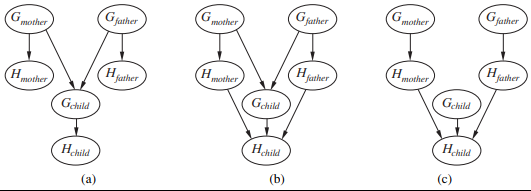
\includegraphics{./immagini/eshandedness}
\end{center}

\begin{itemize}
	\item Quale delle tre reti esprime questa proprietà?
	\[ P(G_{Father}, G_{Mother}, G_{Child}) = P(G_{Mother}) \cdot P(G_{Father}) \cdot P(G_{Child})\]
\end{itemize}

La rete (c) perchè nella terza le tre probabilità sono indipendenti.

\begin{itemize}
	\item Quali delle tre reti esprime le condizioni descritte dal testo del problema?
\end{itemize}

La prima e la seconda, la terza non va bene perchè non rappresenta il fatto che il gene del figlio venga ereditato dai genitori.

\begin{itemize}
	\item Quale delle tre reti descrive al meglio l'ipotesi descritte nel problema?
\end{itemize}

	La prima: la manualità dei genitori non influenza direttamente la manualità dei figli per cui la seconda rete non è corretta.

\begin{itemize}
	\item Qual è la CPT per per \(G_C\) per la prima rete?
\end{itemize}
Quando nei genitori c'è sia L che R m non viene considerato perchè è equivalente la probabilità che si passi da L -> R o da R -> L \\

\begin{tabular}{|c|c|c|l|}
	\hline
	GMother & GFather & P(GChild = L | ...) & P(GChild  = R | ...) \\ \hline
	L       & L       & 1-m                 & m                    \\ \hline
	L       & R       & 0.5                 & 0.5                  \\ \hline
	R       & L       & 0.5                 & 0.5                  \\ \hline
	R       & R       & m                   & 1-m                  \\ \hline
\end{tabular}

\end{document}